\documentclass[]{article}
\usepackage{lmodern}
\usepackage{amssymb,amsmath}
\usepackage{ifxetex,ifluatex}
\usepackage{fixltx2e} % provides \textsubscript
\ifnum 0\ifxetex 1\fi\ifluatex 1\fi=0 % if pdftex
  \usepackage[T1]{fontenc}
  \usepackage[utf8]{inputenc}
\else % if luatex or xelatex
  \ifxetex
    \usepackage{mathspec}
  \else
    \usepackage{fontspec}
  \fi
  \defaultfontfeatures{Ligatures=TeX,Scale=MatchLowercase}
\fi
% use upquote if available, for straight quotes in verbatim environments
\IfFileExists{upquote.sty}{\usepackage{upquote}}{}
% use microtype if available
\IfFileExists{microtype.sty}{%
\usepackage{microtype}
\UseMicrotypeSet[protrusion]{basicmath} % disable protrusion for tt fonts
}{}
\usepackage[margin=1in]{geometry}
\usepackage{hyperref}
\hypersetup{unicode=true,
            pdfborder={0 0 0},
            breaklinks=true}
\urlstyle{same}  % don't use monospace font for urls
\usepackage{color}
\usepackage{fancyvrb}
\newcommand{\VerbBar}{|}
\newcommand{\VERB}{\Verb[commandchars=\\\{\}]}
\DefineVerbatimEnvironment{Highlighting}{Verbatim}{commandchars=\\\{\}}
% Add ',fontsize=\small' for more characters per line
\usepackage{framed}
\definecolor{shadecolor}{RGB}{248,248,248}
\newenvironment{Shaded}{\begin{snugshade}}{\end{snugshade}}
\newcommand{\KeywordTok}[1]{\textcolor[rgb]{0.13,0.29,0.53}{\textbf{#1}}}
\newcommand{\DataTypeTok}[1]{\textcolor[rgb]{0.13,0.29,0.53}{#1}}
\newcommand{\DecValTok}[1]{\textcolor[rgb]{0.00,0.00,0.81}{#1}}
\newcommand{\BaseNTok}[1]{\textcolor[rgb]{0.00,0.00,0.81}{#1}}
\newcommand{\FloatTok}[1]{\textcolor[rgb]{0.00,0.00,0.81}{#1}}
\newcommand{\ConstantTok}[1]{\textcolor[rgb]{0.00,0.00,0.00}{#1}}
\newcommand{\CharTok}[1]{\textcolor[rgb]{0.31,0.60,0.02}{#1}}
\newcommand{\SpecialCharTok}[1]{\textcolor[rgb]{0.00,0.00,0.00}{#1}}
\newcommand{\StringTok}[1]{\textcolor[rgb]{0.31,0.60,0.02}{#1}}
\newcommand{\VerbatimStringTok}[1]{\textcolor[rgb]{0.31,0.60,0.02}{#1}}
\newcommand{\SpecialStringTok}[1]{\textcolor[rgb]{0.31,0.60,0.02}{#1}}
\newcommand{\ImportTok}[1]{#1}
\newcommand{\CommentTok}[1]{\textcolor[rgb]{0.56,0.35,0.01}{\textit{#1}}}
\newcommand{\DocumentationTok}[1]{\textcolor[rgb]{0.56,0.35,0.01}{\textbf{\textit{#1}}}}
\newcommand{\AnnotationTok}[1]{\textcolor[rgb]{0.56,0.35,0.01}{\textbf{\textit{#1}}}}
\newcommand{\CommentVarTok}[1]{\textcolor[rgb]{0.56,0.35,0.01}{\textbf{\textit{#1}}}}
\newcommand{\OtherTok}[1]{\textcolor[rgb]{0.56,0.35,0.01}{#1}}
\newcommand{\FunctionTok}[1]{\textcolor[rgb]{0.00,0.00,0.00}{#1}}
\newcommand{\VariableTok}[1]{\textcolor[rgb]{0.00,0.00,0.00}{#1}}
\newcommand{\ControlFlowTok}[1]{\textcolor[rgb]{0.13,0.29,0.53}{\textbf{#1}}}
\newcommand{\OperatorTok}[1]{\textcolor[rgb]{0.81,0.36,0.00}{\textbf{#1}}}
\newcommand{\BuiltInTok}[1]{#1}
\newcommand{\ExtensionTok}[1]{#1}
\newcommand{\PreprocessorTok}[1]{\textcolor[rgb]{0.56,0.35,0.01}{\textit{#1}}}
\newcommand{\AttributeTok}[1]{\textcolor[rgb]{0.77,0.63,0.00}{#1}}
\newcommand{\RegionMarkerTok}[1]{#1}
\newcommand{\InformationTok}[1]{\textcolor[rgb]{0.56,0.35,0.01}{\textbf{\textit{#1}}}}
\newcommand{\WarningTok}[1]{\textcolor[rgb]{0.56,0.35,0.01}{\textbf{\textit{#1}}}}
\newcommand{\AlertTok}[1]{\textcolor[rgb]{0.94,0.16,0.16}{#1}}
\newcommand{\ErrorTok}[1]{\textcolor[rgb]{0.64,0.00,0.00}{\textbf{#1}}}
\newcommand{\NormalTok}[1]{#1}
\usepackage{graphicx,grffile}
\makeatletter
\def\maxwidth{\ifdim\Gin@nat@width>\linewidth\linewidth\else\Gin@nat@width\fi}
\def\maxheight{\ifdim\Gin@nat@height>\textheight\textheight\else\Gin@nat@height\fi}
\makeatother
% Scale images if necessary, so that they will not overflow the page
% margins by default, and it is still possible to overwrite the defaults
% using explicit options in \includegraphics[width, height, ...]{}
\setkeys{Gin}{width=\maxwidth,height=\maxheight,keepaspectratio}
\IfFileExists{parskip.sty}{%
\usepackage{parskip}
}{% else
\setlength{\parindent}{0pt}
\setlength{\parskip}{6pt plus 2pt minus 1pt}
}
\setlength{\emergencystretch}{3em}  % prevent overfull lines
\providecommand{\tightlist}{%
  \setlength{\itemsep}{0pt}\setlength{\parskip}{0pt}}
\setcounter{secnumdepth}{0}
% Redefines (sub)paragraphs to behave more like sections
\ifx\paragraph\undefined\else
\let\oldparagraph\paragraph
\renewcommand{\paragraph}[1]{\oldparagraph{#1}\mbox{}}
\fi
\ifx\subparagraph\undefined\else
\let\oldsubparagraph\subparagraph
\renewcommand{\subparagraph}[1]{\oldsubparagraph{#1}\mbox{}}
\fi

%%% Use protect on footnotes to avoid problems with footnotes in titles
\let\rmarkdownfootnote\footnote%
\def\footnote{\protect\rmarkdownfootnote}

%%% Change title format to be more compact
\usepackage{titling}

% Create subtitle command for use in maketitle
\newcommand{\subtitle}[1]{
  \posttitle{
    \begin{center}\large#1\end{center}
    }
}

\setlength{\droptitle}{-2em}

  \title{}
    \pretitle{\vspace{\droptitle}}
  \posttitle{}
    \author{}
    \preauthor{}\postauthor{}
    \date{}
    \predate{}\postdate{}
  
\usepackage{float}

\begin{document}

\begin{centering}

\vspace*{5 cm}

\Huge

{\bf Introducción a Python}

\vspace{3 cm}

\Large
Marco Andrés Vázquez Hernández

\vspace{1 cm}
\normalsize
Práctica 2. 

Agosto de 2018

\normalsize
Instituto Politécnico Nacional


\end{centering}

\newpage

\section{Descripción}\label{descripcion}

\begin{enumerate}
\def\labelenumi{\arabic{enumi}.}
\item
  Leer el archivo ``TodasLasNoticias.csv'' y pasarlo a un archivo JSON.
  El objeto contendrá una lista con un diccionario por cada posición,
  donde cada diccionario tendrá cinco llaves: I Fecha, II Título, III
  url IV Descripción, V Categoría
\item
  Guardar el archivo JSON con el nombre ``noticias.json''
\end{enumerate}

Imágen del código:

\begin{figure}[htbp]
\centering
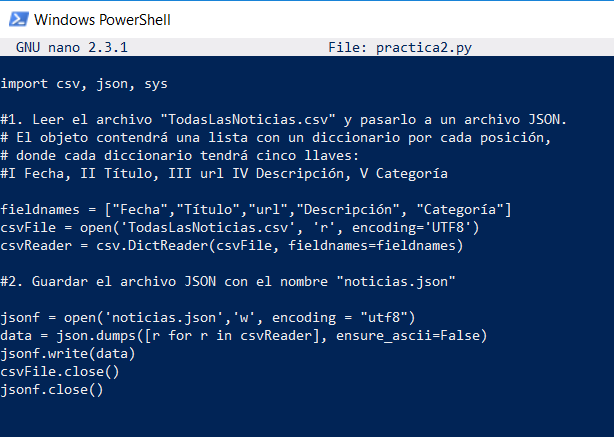
\includegraphics{practica2py.png}
\end{figure}

Ejecución del código:

\begin{figure}[htbp]
\centering
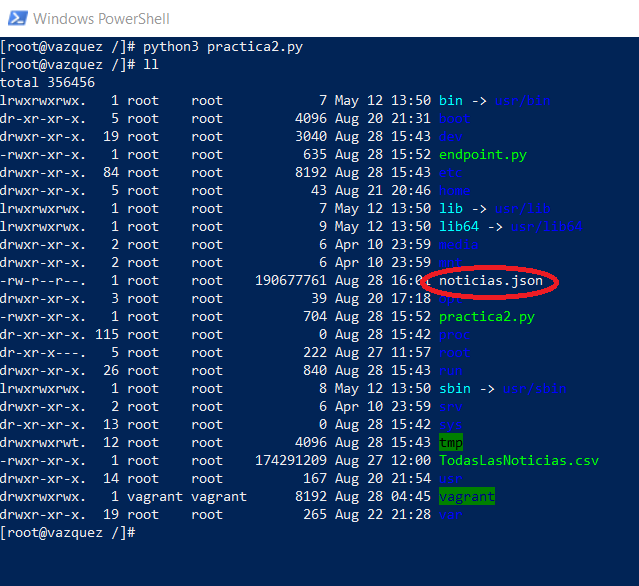
\includegraphics{practica2pyex.png}
\end{figure}

\newpage

\section{Endpoint}\label{endpoint}

\begin{enumerate}
\def\labelenumi{\arabic{enumi}.}
\setcounter{enumi}{2}
\tightlist
\item
  Hacer un endpoint que reciba una petición de tipo GET con el parámetro
  ``categoría'' para que retorne las noticias correspondientes al
  parámetro dado.
\end{enumerate}

El código para esto es:

\begin{figure}[htbp]
\centering
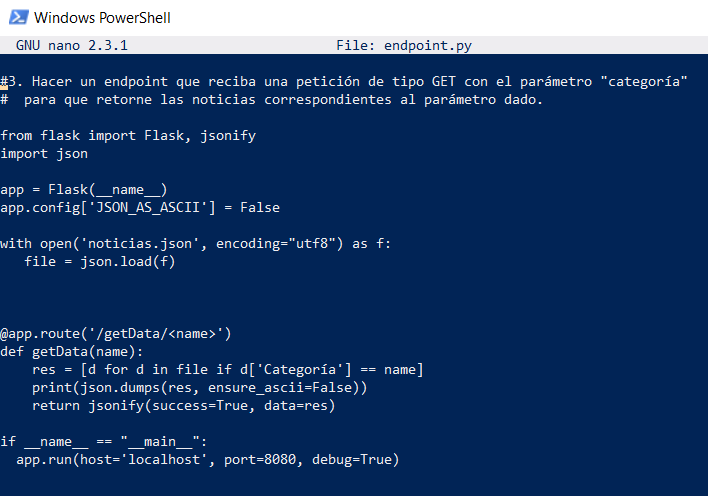
\includegraphics{endpointpy.png}
\end{figure}

Para la creación de un endpoint se tiene que tener instalado pip, flask
y virtualenv y otros requisitos:

\begin{Shaded}
\begin{Highlighting}[]
\FunctionTok{sudo}\NormalTok{ yum install python-pip python-devel gcc nginx}
\FunctionTok{sudo}\NormalTok{ yum install python34-setuptools}
\FunctionTok{sudo}\NormalTok{ easy_install-3.4 pip}
\FunctionTok{sudo}\NormalTok{ pip3 install flask}
\FunctionTok{sudo}\NormalTok{ pip install virtualenv}
\end{Highlighting}
\end{Shaded}

Despues se crea una instancia virtual de Python para el proyecto
endpoint.py:

\begin{Shaded}
\begin{Highlighting}[]
\FunctionTok{sudo}\NormalTok{ virtualenv endpointenv}
\end{Highlighting}
\end{Shaded}

NOTA: Para el caso de Vagrant sobre Windows, el entorno virtual sólo se
puede crear sobre /. También se tiene que configurar el archivo
Vagrantfile tal que contenga la siguiente linea:

\begin{Shaded}
\begin{Highlighting}[]
\ExtensionTok{config.vm.network} \StringTok{"forwarded_port"}\NormalTok{, guest: 8080, host: 8080}
\end{Highlighting}
\end{Shaded}

La ejecución del código:

\begin{figure}[htbp]
\centering
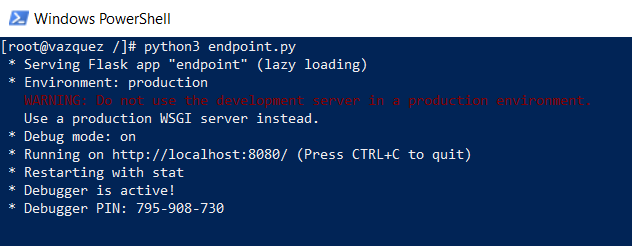
\includegraphics{endpointpyex.png}
\end{figure}

\newpage

Para probar que el servicio funciona se puede ejecutar el comando:

\begin{Shaded}
\begin{Highlighting}[]
 \ExtensionTok{curl}\NormalTok{ -i -X GET http://localhost:8080/getData/Yucatan }\KeywordTok{|} \FunctionTok{head}\NormalTok{ -n 30}
\end{Highlighting}
\end{Shaded}

Nota: Usar tmux.

Debe de arrojar:

\begin{figure}[htbp]
\centering
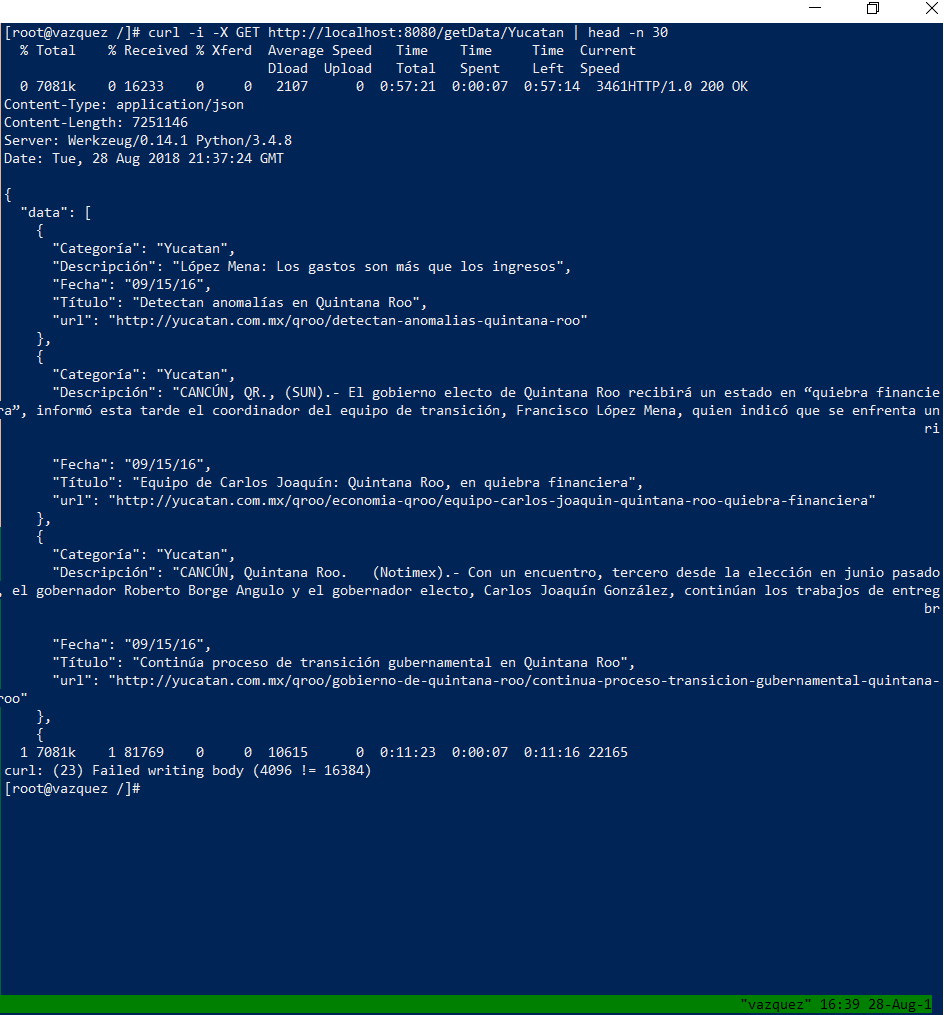
\includegraphics{getcommand.png}
\end{figure}

\newpage

Desde un navegador también se debe poder checar bajo la dirección
\url{http://localhost:8080/getData/}:

\begin{figure}[htbp]
\centering
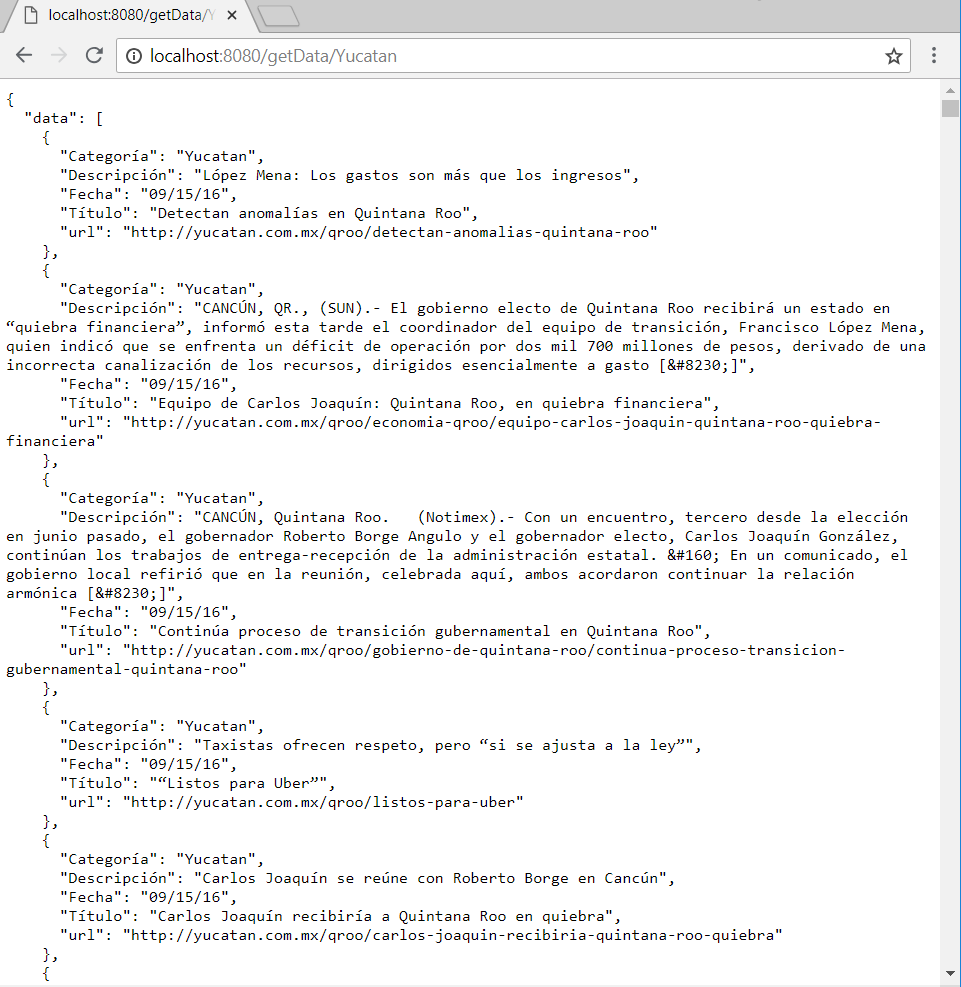
\includegraphics{getweb.png}
\end{figure}

Nota: Para una aplicación flask desde una maquina virtual de Vagrant
sobre Windows hay configuraciones adicionales y posibles bugs que aquí
no se detallan.


\end{document}
